%%
% This is an Overleaf template for presentations
% using the TUM Corporate Desing https://www.tum.de/cd
%
% For further details on how to use the template, take a look at our
% GitLab repository and browse through our test documents
% https://gitlab.lrz.de/latex4ei/tum-templates.
%
% The tumbeamer class is based on the beamer class.
% If you need further customization please consult the beamer class guide
% https://ctan.org/pkg/beamer.
% Additional class options are passed down to the base class.
%
% If you encounter any bugs or undesired behaviour, please raise an issue
% in our GitLab repository
% https://gitlab.lrz.de/latex4ei/tum-templates/issues
% and provide a description and minimal working example of your problem.
%%

%\makeatletter
%\def\input@path{{../beamer/}}
%\makeatother

\documentclass[
  german,            % define the document language (english, german)
  aspectratio=169,    % define the aspect ratio (169, 43)
  % handout=2on1,       % create handout with multiple slides (2on1, 4on1)
  % partpage=false,     % insert page at beginning of parts (true, false)
  % sectionpage=true,   % insert page at beginning of sections (true, false)
]{tumbeamer}


% load additional packages
\usepackage{booktabs}
\usepackage{graphicx}
\usepackage{tikz}
\usepackage{url}
\usepackage{pgfplots}
\usepackage{hyperref}
\usepackage{pmboxdraw}
\usepackage{float}
\usepackage{listings}
\usepackage{circuitikz}
%\usepackage[european]{circuitikz}
\usepackage{babel}[ngerman]
\usepackage{csquotes}[autostyle]
\usepackage[useregional]{datetime2}

% image path
\graphicspath{ {./resources/} }

% presentation metadata
\title{Übung 13: Parallelisierung}
\subtitle{Einführung in die Rechnerarchitektur}
\author{Niklas Ladurner}

\institute{\theChairName\\\theDepartmentName\\\theUniversityName}
\date{\DTMdisplaydate{2024}{1}{26}{-1}}

\footline{\insertauthor~|~\insertshorttitle~|~\insertshortdate}


% macro to configure the style of the presentation
\TUMbeamersetup{
  title page = TUM tower,         % style of the title page
  part page = TUM toc,            % style of part pages
  section page = TUM toc,         % style of section pages
  content page = TUM more space,  % style of normal content pages
  tower scale = 1.0,              % scaling factor of TUM tower (if used)
  headline = TUM threeliner,      % which variation of headline to use
  footline = TUM default,         % which variation of footline to use
  % configure on which pages headlines and footlines should be printed
  headline on = {title page},
  footline on = {every page, title page=false},
}

% available frame styles for title page, part page, and section page:
% TUM default, TUM tower, TUM centered,
% TUM blue default, TUM blue tower, TUM blue centered,
% TUM shaded default, TUM shaded tower, TUM shaded centered,
% TUM flags
%
% additional frame styles for part page and section page:
% TUM toc
%
% available frame styles for content pages:
% TUM default, TUM more space
%
% available headline options:
% TUM empty, TUM oneliner, TUM twoliner, TUM threeliner, TUM logothreeliner
%
% available footline options:
% TUM empty, TUM default, TUM infoline


\begin{document}

\maketitle

\begin{frame}[c]{}{}
  \begin{center}
    \LARGE  Durchzählen!
  \end{center}
\end{frame}

\begin{frame}[c]{}{}
  \begin{center}
    \LARGE  Keine Garantie für die Richtigkeit der Tutorfolien: Bei Unklarheiten/Unstimmigkeiten
    haben VL/ZÜ-Folien Recht!
  \end{center}
\end{frame}

\begin{frame}[fragile, c]{Parallelisierungstechniken}{}
  \begin{columns}[c]
    \begin{column}{0.5\textwidth}
      \begin{itemize}
        \item Single-Threaded Rechenleistung immer weiter durch physikalische Limits eingeschränkt
        \item Optimierungen: Pipelining, Out-of-Order-Processing, Ausnutzen von Parallelität
        \item SIMD: Eine Instruktion, die gleichzeitig auf mehrere Daten ausgeführt wird (mehr dazu in GRA)
        \item Multithreading/Mehrkernsysteme $\rightarrow$ mögliche Cache-Inkonsistenzen
      \end{itemize}
    \end{column}
    \begin{column}{0.5\textwidth}
      \begin{center}
        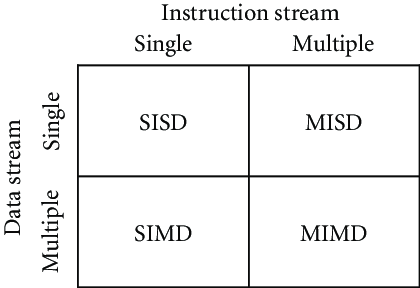
\includegraphics[width=0.7\textwidth]{w13_flynn.png}
      \end{center}
      \centering
      \tiny{Quelle: A Taxonomy of Reconfigurable Single-/Multiprocessor\\Systems-on-Chip}
    \end{column}
  \end{columns}
\end{frame}

\begin{frame}[fragile, c]{MSI/MESI}{}
  \begin{columns}[c]
    \begin{column}{0.5\textwidth}
      \begin{itemize}
        \item Einführung von Zuständen für Cachezeilen
        \item \textbf{M}odified, (\textbf{E}xclusive), \textbf{S}hared, \textbf{I}nvalid
        \item Erklärung siehe ZÜ
      \end{itemize}
    \end{column}
    \begin{column}{0.5\textwidth}
      \begin{center}
        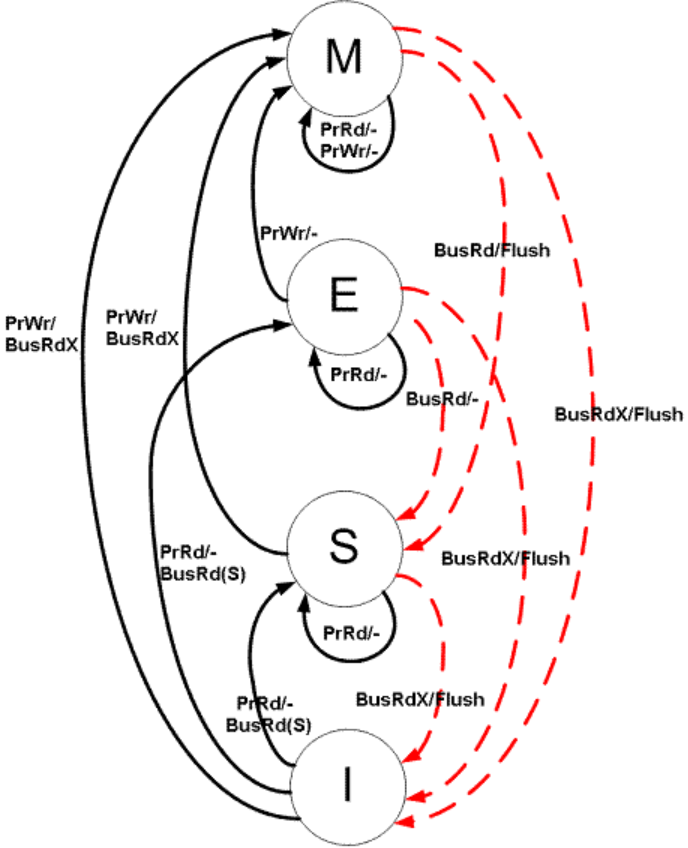
\includegraphics[width=0.7\textwidth]{w13_mesi.png}
      \end{center}
      \centering
      \tiny{Quelle: Jugones55, CC BY-SA 4.0 \href{https://creativecommons.org/licenses/by-sa/4.0}{via Wikimedia Commons}}
    \end{column}
  \end{columns}
\end{frame}


\begin{frame}[c, fragile]{Speedup durch Parallelisierung}{}
  Mit $t_s$ sequentieller Programmteil, $t_p$ paralleler Programmteil, $n$ Anzahl CPU-Kerne
  \begin{itemize}
    \item Amdahl's Law: $s_{\textrm{Amdahl}}(n)=\frac{T}{t_s+\frac{t_p}{n}}$\\
          Gleiche Problemgröße, aufgeteilt auf mehrere Kerne $\rightarrow$ begrenzt durch sequentiellen Anteil
    \item Gustafson's Law: $s_{\textrm{Gustavson}}(n)=\frac{t_s+n\cdot t_p}{T}$\\
          Größeres Problem$\rightarrow$ paralleler Anteil wächst mit Problemgröße, $t_s$ proportional kleiner
    \item Zwei verschiedene Perspektiven, abhängig von Problemszenario verschieden geeignet
  \end{itemize}
\end{frame}

\begin{frame}[fragile, c]{Amdahl's Law: graphische Darstellung}{}
      \begin{center}
        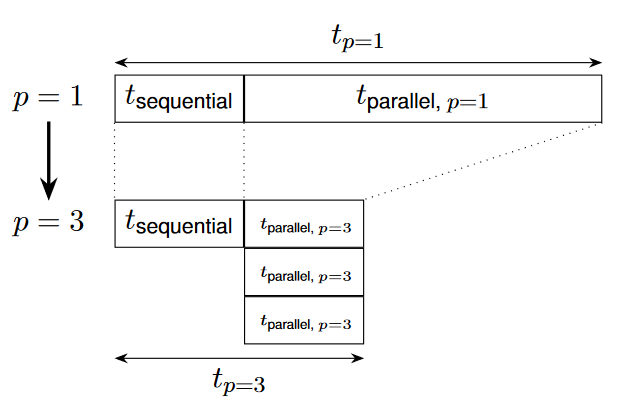
\includegraphics[width=0.65\textwidth]{w13_amdahl.png}
      \end{center}
  \centering
  \tiny{Quelle: Vorlesungsmaterial ERA}
\end{frame}


\begin{frame}[c]{}{}
  \begin{center}
    \LARGE Fragen?
  \end{center}
\end{frame}

\begin{frame}[c, fragile]{Artemis-Hausaufgaben}{}
  \begin{itemize}
    \item H13 - MESI bis 04.02.2024 23:59 Uhr
    \item MESI-Tabelle zu verschiedenen Aktionen ausfüllen
    \item Letzte reguläre Hausaufgabe
    \item \underline{Um den Notenbonus zu erhalten, braucht man also $\ge 0.8\cdot 130 = 104$ Punkte!}
    \item Der Notenbonus wird nur angewandt, wenn die Ausgangsnote besser als 5.0 und nicht 1.0 ist
  \end{itemize}
\end{frame}

\begin{frame}[fragile, c]{Links}{}
  \begin{itemize}
    \item Zulip: \href{https://zulip.in.tum.de/#narrow/stream/1917-ERA-Tutorium---Mi-1600-MI4}{\enquote{ERA Tutorium - Mi-1600-MI4}}
    bzw. \href{https://zulip.in.tum.de/#narrow/stream/1940-ERA-Tutorium---Fr-1100-MW2}{\enquote{ERA Tutorium - Fr-1100-MW2}}
    \item \href{https://de.wikipedia.org/wiki/MESI}{Wikipedia zu MESI}
    \item \href{https://www.educative.io/answers/difference-between-amdahls-and-gustafsons-laws}{Amdahlsches und Gustafsons Gesetz}
  \end{itemize}
\end{frame}

\maketitle

\end{document}
